\subsection{Media Player}
This subsystem is apart of the graphical interface that allows the user to play/stop a song streaming from a third party music service.

\begin{figure}[h!]
	\centering
 	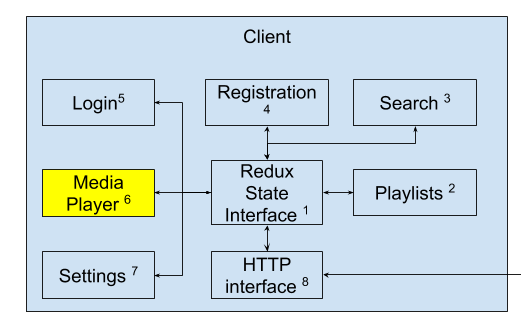
\includegraphics[width=0.60\textwidth]{images/client/client_media.png}
 	\caption{Media player subsystem}
\end{figure}

\subsubsection{Subsystem Hardware}
No hardware is used for this layer. The media player will be a component of the home page which will be hosted on Heroku.

\subsubsection{Subsystem Operating System}
No OS required. The media player will run through supported browsers such as Chrome 42 and Firefox 39.

\subsubsection{Subsystem Software Dependencies}
React.js 16.8.0-alpha.1 is used for the framework and the Fetch API from Mozilla will be used to retrieve song information.

\subsubsection{Subsystem Programming Languages}
JavaScript ES6 will be used.

\subsubsection{Subsystem Data Structures}
A JSON object containing music information will be used to display song information and to stream audio.

\subsubsection{Subsystem Data Processing}
No algorithms used.


\newpage